\documentclass[11pt]{article}

\usepackage[margin=1in]{geometry}
\usepackage{times}
\usepackage[T1]{fontenc}
\usepackage{graphicx}
\usepackage{booktabs}
\usepackage{amsmath}
\usepackage[colorlinks=true,linkcolor=black,citecolor=black,urlcolor=black]{hyperref}
\usepackage{natbib}
\usepackage{caption}
\usepackage{float}

\title{\textbf{VAYAS\thanks{VAYAS is this project's name (Paper 1 of the Vyaskosh series), not a
letter-by-letter acronym.}: An Age-Stratified Zero-Shot Audit of Hindi Speech Recognition}}

\author{Shubham Kumar Gupta \\ \texttt{kshubham04907@gmail.com} \and Sania Gurung \\ \texttt{saniagurung5452@gmail.com}}
\date{}

\begin{document}

\maketitle

\begin{abstract}
We present a zero-shot audit of four automatic speech recognition (ASR) systems for Hindi,
examining whether word- and character-error rates differ by speaker age under a matched-cohort
design. Common Voice Hindi, the most widely used open Hindi ASR benchmark, turns out to have
almost no confirmed elderly speakers once its self-reported age field is actually counted (2 in
their 60s, 0 older, out of 369 speakers). We instead use IndicVoices-R Hindi, a public
spontaneous-speech corpus with genuine elderly (age 60+) representation, comparing 50 elderly
speakers against a duration-matched, same-corpus control cohort randomly sampled from a 318-speaker
pool (313--317 speakers actually drawn, depending on system; Section~\ref{sec:matching}),
across four systems: OpenAI Whisper large-v3, Meta MMS-1B, and two India-specialized models,
AI4Bharat's IndicConformer and IndicWhisper. IndicConformer achieves the lowest error rates by a
wide margin (WER 17.1--18.3\%, CER 5.2--7.6\%); we flag a serious, unresolved caveat on this
result, since AI4Bharat's models are documented elsewhere as trained in part on IndicVoices, the
corpus IndicVoices-R is itself derived from, raising a real train-test contamination risk we
could not rule out. IndicWhisper, also India-specialized, is the weakest performer (WER
46.4--50.5\%); we trace a substantial share of this (about a quarter of the elderly-control gap)
to a decoder repetition-loop failure mode, 16--80x more frequent than in the other three systems,
concentrated on short utterances. Age-cohort effect sizes are small across all four systems
(Cohen's $d < 0.2$ in every case); one nominally significant elderly disadvantage (IndicWhisper,
$p = 0.032$--$0.036$) does not survive correction for multiple comparisons across the eight
system-metric tests, and is below this sample's minimum detectable effect size, so we report it
as suggestive, not confirmed. We tested and ruled out one alternative explanation directly:
re-scoring every clip against a disfluency-free reference transcript (rather than the
disfluency-preserving one used throughout) leaves all eight effect signs, and IndicWhisper's
pattern specifically, essentially unchanged. We release the full zero-shot audit pipeline,
matched-cohort sampling code, and per-clip results.
\end{abstract}

\section{Introduction}

Automatic speech recognition (ASR) systems are increasingly deployed as the primary interface
for voice assistants, transcription tools, and accessibility technology. Prior audits of
commercial ASR in English have found substantial disparities in error rate across demographic
groups defined by race \citep{koenecke2020racial}, and structural audits of other speech and
vision systems have shown that undisclosed performance gaps across a benchmark's underlying
population are common when systems are evaluated only in aggregate \citep{buolamwini2018gender}.
Age is a comparatively under-studied axis for this kind of audit, and Hindi -- despite being
among the most widely spoken languages in the world -- has very little public infrastructure for
answering this question at all: the most commonly used open Hindi ASR benchmark, Common Voice,
turns out to have almost no \emph{confirmed} elderly speakers once its self-reported age field is
actually counted (Section~\ref{sec:data}).

This paper reports a zero-shot audit -- no system is fine-tuned or otherwise modified -- of four
ASR systems on Hindi speech, following the general blueprint of building a benchmark and auditing
existing systems against it rather than training anything new \citep{buolamwini2018gender}, and
adopting the matched-cohort design of \citet{koenecke2020racial}: an elderly group and a
same-source, same-conditions control group, so that age is the only systematic difference between
the two samples being compared. We find one dominant result (a large, consistent quality gap
between systems, whose interpretation is complicated by a training-data contamination risk we
flag but cannot resolve) and one narrower, suggestive but not statistically confirmed signal (a
small elderly disadvantage specific to one system, driven partly, not wholly, by an identifiable
failure mode in its decoder). We treat both as worth reporting in full, including where they fall
short of confirmation: a mostly-null result across three of four systems is not a failure of the
audit, it is information about where an age-based accessibility problem does and does not
currently show up at the sample size this study could run.

\section{Related Work}

\citet{koenecke2020racial} audited five commercial ASR systems on African American Vernacular
English versus white American English using matched speaker cohorts, finding substantially higher
word error rates for Black speakers across every system tested; the matched-cohort design used
here -- same corpus, same recording conditions, one demographic axis varied -- follows that
methodology directly. \citet{buolamwini2018gender} established the broader structural pattern this
work follows: constructing a benchmark with genuine population coverage and auditing already-deployed
systems against it, rather than proposing a new model. \citet{pellegrini2012impact} is the closest
prior study of age effects specifically, examining the impact of age on ASR performance in a
non-English setting; we adopt its motivating question but, as discussed in
Section~\ref{sec:data}, could not replicate its finer decade-level age banding given our source
data's constraints. \citet{thennal2025cer} motivate reporting both WER and CER together
rather than WER alone, since word- and character-level error can diverge in morphologically rich
languages; Hindi's own morphology (case-marked postpositions, extensive compounding) makes this
decomposition relevant here even though the original motivation was a different language family.

On the systems side, this audit covers Whisper \citep{radford2023whisper}, a general-purpose
multilingual encoder-decoder model; MMS \citep{pratap2023mms}, Meta's massively multilingual
CTC-based system; and two Hindi-specialized systems from AI4Bharat, IndicConformer
\citep{indicconformer2025} and IndicWhisper \citep{bhogale2023vistaar}, both fine-tuned or trained
specifically for Indian languages. Both AI4Bharat systems draw, directly or indirectly, on
IndicVoices \citep{indicvoices2024} as training data, a fact with direct consequences for this
audit's own eval corpus (Section~\ref{sec:contamination}).

\section{Data}
\label{sec:data}

\subsection{Source selection}

We initially considered Mozilla Common Voice Hindi (\texttt{cv-corpus-26.0-2026-06-12},
validated split) as the elderly-cohort source, since it is the most widely cited open Hindi ASR
corpus and provides decade-level age brackets. Counting its validated split directly, however,
shows this is not viable: of 369 total speakers, 145 fall in the under-60 control range, 222 left
the (optional, self-reported) age field blank, and only \textbf{2} speakers are confirmed aged in
their 60s, with \textbf{zero} confirmed in their 70s or 80s. Applying an n$\,\geq\,$8-speakers-per-band
stopping rule, every elderly band fails outright.

We therefore used \textbf{IndicVoices-R Hindi} \citep{indicvoicesr}, the Hindi subset of
AI4Bharat's IndicVoices-R corpus, as the source of record for both the elderly and control
cohorts. A full, column-selective read of all 10 parquet shards (368 unique speakers, 26,318
utterances total, no audio decoded during this scan) gives real, exact per-age-band counts:

\begin{table}[H]
\centering
\caption{IndicVoices-R Hindi: real speaker and utterance counts by age band.}
\label{tab:datacounts}
\begin{tabular}{lrr}
\toprule
\textbf{Age group} & \textbf{Speakers} & \textbf{Utterances} \\
\midrule
18--30 & 128 & 8{,}778 \\
30--45 & 117 & 8{,}503 \\
45--60 & 73 & 5{,}138 \\
\textbf{60+} & \textbf{50} & \textbf{3{,}899} \\
\midrule
Total & 368 & 26{,}318 \\
\bottomrule
\end{tabular}
\end{table}

The elderly (60+) band clears the n$\,\geq\,$8 threshold with wide margin, and the combined
under-60 pool (318 speakers) is more than sufficient for a same-corpus, duration-matched control
cohort (Section~\ref{sec:matching}). Figure~\ref{fig:cohort} and Figure~\ref{fig:datasetcompare}
summarize this comparison.

\begin{figure}[H]
\centering
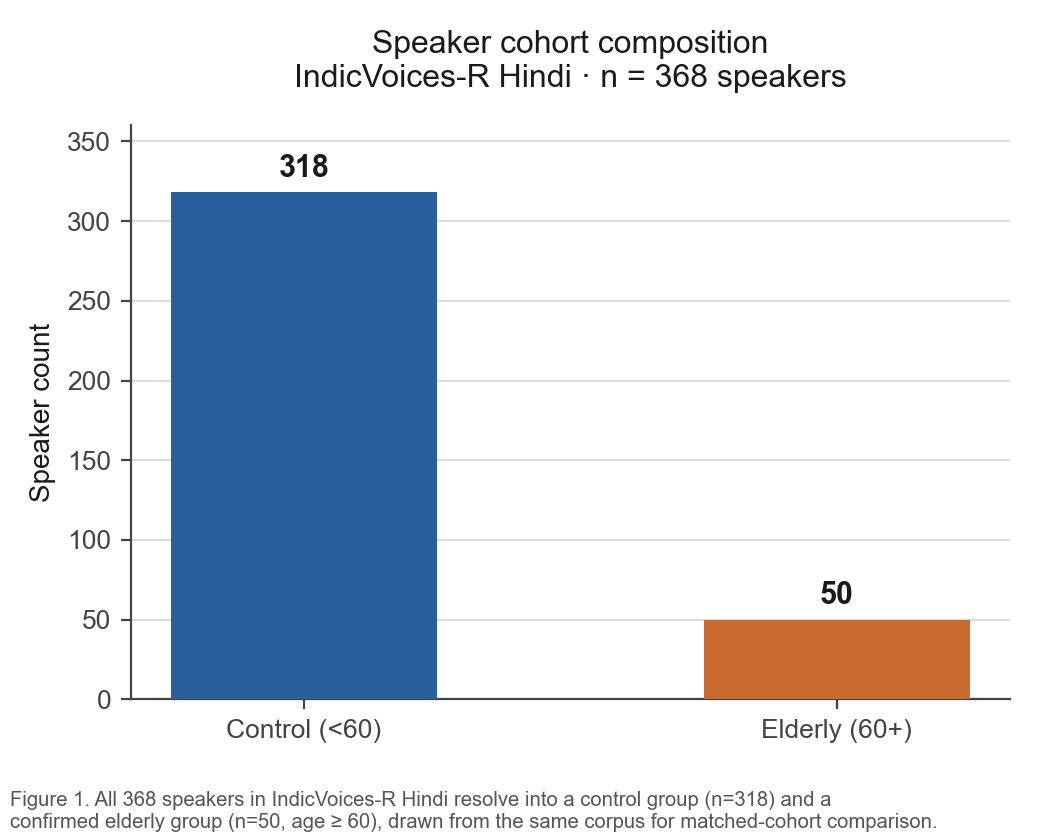
\includegraphics[width=0.62\linewidth]{figures/figure1_cohort.png}
\caption{Full speaker cohort composition, IndicVoices-R Hindi (n=368).}
\label{fig:cohort}
\end{figure}

\begin{figure}[H]
\centering
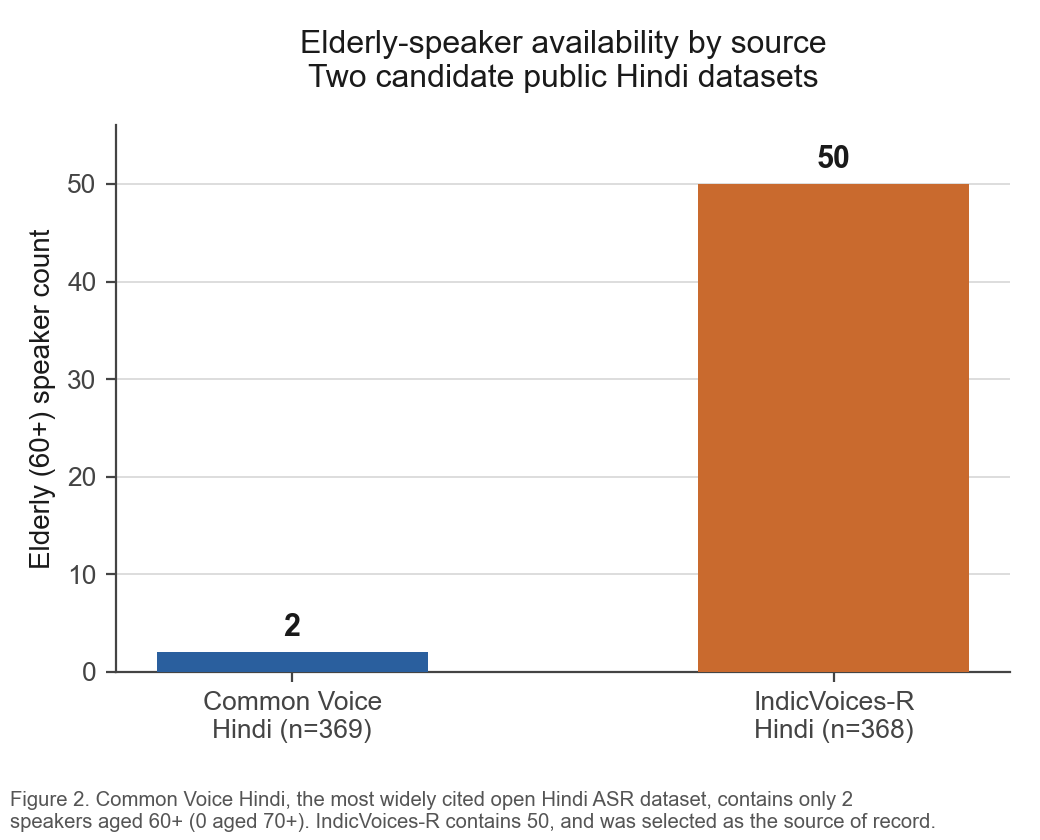
\includegraphics[width=0.62\linewidth]{figures/figure2_dataset_comparison.png}
\caption{Elderly-speaker availability: Common Voice Hindi vs.\ IndicVoices-R Hindi.}
\label{fig:datasetcompare}
\end{figure}

\subsection{Age-band resolution and speech type}

IndicVoices-R's \texttt{age\_group} field is a 4-class label (\texttt{18-30}, \texttt{30-45},
\texttt{45-60}, \texttt{60+}) with no finer resolution available from public metadata. Unlike
the decade-level scheme used by \citet{pellegrini2012impact} and originally targeted by this
project, there is no way to distinguish speakers in their 60s, 70s, or 80s from this source. We
therefore report a single collapsed elderly (60+) band against a single control (\textless\,60)
band, rather than the finer scheme we had originally intended; this is a real resolution loss we
state plainly rather than silently substituting a coarser claim for a finer one.

We manually inspected a sample of \texttt{verbatim}/\texttt{normalized}/\texttt{task\_name} fields
to confirm speech type before treating this as a spontaneous-speech corpus. Two signals both
indicate genuine spontaneous, topic-elicited speech rather than read-aloud script: (1)
\texttt{task\_name} values are topic prompts (``KYP - Cooking'', ``Daily Life'', ``Alexa
Commands''), not transcript references; and (2) \texttt{verbatim} preserves colloquial spelling
and at least one visible disfluency/false-start that the cleaned \texttt{normalized} field
scrubs. We use \texttt{verbatim} as the gold reference throughout, since it is the field that
actually preserves what a spontaneous-speech evaluation should measure against.

One caveat carries through every result in this paper: IndicVoices-R applies a speech-enhancement
(denoising/dereverberation) preprocessing step before release, which may suppress some of the
acoustic degradation an age-based audit is trying to measure. We flag this as a standing
limitation (Section~\ref{sec:limitations}), not a resolved issue.

\subsection{Cohort construction}
\label{sec:matching}

The elderly cohort is all 50 confirmed 60+ speakers in IndicVoices-R Hindi. The control cohort is
drawn from the same corpus's 318-speaker under-60 pool via duration-matched random sampling: control
clips are shuffled and greedily accumulated until their total duration meets or exceeds the
elderly cohort's total duration, so that the two cohorts are comparable in scale as well as
source. Sourcing both cohorts from the same corpus, rather than pairing IndicVoices-R elderly
speakers against a Common Voice control group, is what makes this a matched-cohort design in the
sense of \citet{koenecke2020racial}: the only systematic difference between the two samples is
age, not platform, recording setup, or elicitation protocol.

Two of the four systems (MMS, IndicConformer) were run against the full elderly pool (3,899
clips) plus an equal-duration control sample (3,787 clips), 7,686 clips total. The other two
(Whisper large-v3, IndicWhisper) measured 2--4x slower than real-time on the GPUs available for
this study (an RTX 3050 laptop GPU, 4GB VRAM, for development; Kaggle-hosted NVIDIA P100/T4
instances for the full batch runs), so were run against a smaller, still duration-matched,
non-overlapping union of
three sampling passes (elderly and control positions from each earlier pass were explicitly
excluded before sampling the next, using the same deterministic scan order and a fresh random
seed per pass -- see \texttt{scripts/} in the released code, which recovers each pass's exact
sample by replaying its seed rather than only checking for accidental overlap after the fact):
4,807 unique clips total, comprising 2,434 elderly and 2,373 control clips.

Duration-matching alone does not equalize per-speaker clip counts, and it does not. Elderly
speakers contribute far more clips each than control speakers: 77.98 clips/speaker (elderly) vs.\
11.95 (control) in the MMS/IndicConformer pool, and 48.68 vs.\ 7.58 in the Whisper/IndicWhisper
pool. Since our statistics aggregate to one mean per speaker before computing confidence intervals
and effect sizes (Section~\ref{sec:stats}), control speaker-level means are computed from far
fewer clips each and are correspondingly noisier -- this is the direct cause of at least one
visibly wide control-cohort confidence interval in Table~\ref{tab:summary} (IndicConformer
control CER). Age remains the only \emph{demographic} axis deliberately varied between cohorts,
but it is not the only difference in how each cohort's statistics are computed, and we do not
claim otherwise. Balancing clips per speaker, not just total duration, is the clear next step for
this sampling design (Section~\ref{sec:limitations}).

\subsection{Training-data contamination risk}
\label{sec:contamination}

A serious caveat applies specifically to IndicConformer and IndicWhisper, and we did not have it
fully resolved before running the audit. IndicVoices-R, this paper's evaluation corpus, is
explicitly described by its own authors as derived from IndicVoices \citep{indicvoices2024} via an
audio-restoration pipeline (demixing, dereverberation, denoising) applied to the same underlying
recordings, not an independently collected corpus \citep{indicvoicesr}. Publicly available
AI4Bharat documentation states that their ASR models, including IndicWav2Vec and IndicWhisper, are
trained in part on IndicVoices; we could not obtain an authoritative, model-specific statement
confirming or ruling out IndicConformer's exact training set, despite checking its Hugging Face
model card, its GitHub organization, and AI4Bharat's own ASR project page, none of which publish a
dataset-level training manifest.

This means IndicConformer's result in this paper cannot be presented as a clean zero-shot
comparison without qualification: if its training data included IndicVoices, it may have seen the
same underlying recordings and transcripts as some or all of this paper's evaluation clips
(post-enhancement audio, pre-enhancement audio, or both), which would inflate its apparent accuracy
relative to the two systems in this audit with no plausible IndicVoices exposure (Whisper large-v3,
MMS). One partial, non-conclusive counter-data-point: IndicConformer also produced an exact-match
transcript on a single Common Voice Hindi clip during pilot validation (a corpus wholly unrelated
to IndicVoices), suggesting at least some of its accuracy is not corpus-specific -- but a single
clip cannot settle a corpus-level contamination question, and we do not treat it as doing so.
Given this, we report IndicConformer's result descriptively rather than causally: it is the
best-performing system \emph{on this benchmark, as measured}, and we explicitly do not claim this
reflects a fair, contamination-free zero-shot comparison against the other three systems. Framing
its advantage as an architecture or training-recipe insight (rather than a possible data-leakage
artifact) is not supportable without the speaker- or utterance-level training manifest AI4Bharat
has not published, and we do not make that framing (see Section~\ref{sec:discussion}).

\section{Methodology}

\subsection{Systems audited}
\label{sec:systems}

All four systems are run zero-shot: no fine-tuning, no prompt engineering beyond specifying the
target language where the API supports it.

\begin{itemize}
\item \textbf{Whisper large-v3} \citep{radford2023whisper} (\texttt{openai/whisper-large-v3},
$\sim$1.55B parameters): general-purpose multilingual encoder-decoder, called directly via
\texttt{Whisper\allowbreak ForConditionalGeneration} rather than the higher-level \texttt{pipeline()} wrapper,
after the latter surfaced three separate real integration bugs during development (a missing
system \texttt{ffmpeg} dependency, a \texttt{torchcodec} library mismatch, and a genuine
\texttt{transformers} bug in its dict-input preprocessing path). No explicit beam size,
temperature-fallback, or repetition-penalty configuration was set beyond library defaults; this
gap in disclosure applies equally to IndicWhisper below and is discussed as a limitation
(Section~\ref{sec:limitations}) directly relevant to Section~\ref{sec:degenerate}.
\item \textbf{MMS-1B} \citep{pratap2023mms} (\texttt{facebook/mms-1b-all}, $\sim$1B parameters):
CTC-based, part of Meta's Massively Multilingual Speech project. MMS ships one model with
per-language adapter weights rather than one checkpoint per language; the Hindi adapter is loaded
explicitly via \texttt{processor.\allowbreak tokenizer.\allowbreak set\_target\_lang("hin")} and
\texttt{model.\allowbreak load\_adapter("hin")} before every transcription call.
\item \textbf{IndicConformer} \citep{indicconformer2025}
(\texttt{ai4bharat/\allowbreak indic-conformer-\allowbreak 600m-multilingual}, 600M parameters):
AI4Bharat's Conformer-based multilingual Indic ASR model, run with its CTC
decoding head (the model also supports RNNT decoding; CTC is what this audit used throughout).
\item \textbf{IndicWhisper} \citep{bhogale2023vistaar}: AI4Bharat's Hindi Whisper fine-tune,
distributed as a direct checkpoint archive (not a standard Hugging Face Hub repository) per the
Vistaar project. That archive ships \emph{two} Hindi checkpoints, fine-tuned from different
Whisper base sizes; we confirmed via each checkpoint's own \texttt{config.json} that this audit
used \texttt{whisper-large-hi-noldcil} ($d_{model}=1280$, 32 encoder and 32 decoder layers,
matching Whisper large's architecture, $\sim$1.55B parameters), not the archive's other
\texttt{whisper-medium-hi\_alldata\_multigpu} checkpoint ($d_{model}=1024$, 24+24 layers,
$\sim$769M parameters). We flag this deliberately: our original loading code selected whichever
checkpoint a directory scan happened to return first, which is filesystem-order-dependent and was
not a considered choice at the time -- we verified after the fact which one actually ran, and have
since fixed the loader to select explicitly rather than by scan order.
\end{itemize}

Two further systems in the originally planned seven-system set were excluded after real,
documented attempts rather than assumption: IndicWav2Vec's LM-decoding dependency
(\texttt{pyctcdecode}$\rightarrow$\texttt{kenlm}) does not build against the Python version used
in this environment, and Meta's Omnilingual ASR ships no Windows-compatible native backend wheel
at all. Both are platform gaps in the development environment used for this study, not judgments
that the systems are unusable in principle. A fifth system, Sarvam (a billed API), remains
in-scope but deferred pending an explicit cost decision, and is not included in the results below.

\subsection{Metrics}
\label{sec:metrics}

For every clip with a non-empty gold reference, we compute Word Error Rate (WER) and Character
Error Rate (CER) via \texttt{jiwer} \citep{jiwer}, using its default whitespace word tokenization
and raw character-sequence comparison (no Hindi-specific text normalization is applied; this is a
documented choice, not an oversight). We additionally report the WER$-$CER divergence
\citep{thennal2025cer}, per-clip substitution/insertion/deletion counts, and a speaking-rate
proxy (reference word count divided by clip duration).

We use IndicVoices-R's \texttt{verbatim} field as the gold reference throughout, since it
preserves disfluencies and false starts rather than the cleaned \texttt{normalized} field. This is
a deliberate choice for measuring spontaneous-speech ASR, but it has a real methodological
consequence: no system in this audit is trained to emit disfluencies, so any age-related
difference in disfluency rate could in principle produce a WER/CER gap attributable to reference
style rather than acoustic recognition failure -- the same direction this paper's central
hypothesis (elderly speech is harder to recognize) would also predict. We tested this directly by
re-scoring every clip against \texttt{normalized} references and recomputing every effect size in
Table~\ref{tab:effects}: all 8 effects keep the same sign under both reference styles, and
IndicWhisper's WER/CER pattern in particular is essentially unchanged ($d=0.136$/$0.181$
normalized vs.\ $0.139$/$0.187$ verbatim; still nominally significant, still short of surviving
Benjamini--Hochberg correction, under both scorings). The disfluency confound does not explain away
this paper's age-effect signal, which is a real strengthening of the IndicWhisper result even
though it remains statistically suggestive rather than confirmed (Section~\ref{sec:stats}).

\subsection{Statistics}
\label{sec:stats}

Every aggregate statistic below is reported as an \texttt{(estimate, CI\_low, CI\_high, n)} tuple,
never a bare point estimate.
Per-clip metrics are first aggregated to one mean value per speaker (not pooled across clips
directly), since multiple clips from the same speaker are not independent observations; 95\%
confidence intervals are then obtained via bootstrap resampling of speakers (10,000 resamples).
Elderly-vs-control effect sizes are reported as both Cohen's $d$ (parametric, mean-based) and a
rank-biserial correlation derived from a two-sided Mann-Whitney U test (nonparametric, robust to
skew) on the same per-speaker distributions, with $p$-values from the same test. With 4 systems
$\times$ 2 metrics, this paper runs 8 such tests; we apply a Benjamini--Hochberg correction across
all 8 and report both raw and corrected $p$-values (Table~\ref{tab:effects}), rather than letting
the smallest raw $p$-values stand uncorrected. We also report each test's minimum detectable
effect (MDE) at 80\% power given its actual sample sizes, since a null result from an
underpowered test is not evidence of no effect.

\section{Results}

\subsection{Error rate by system}

Figure~\ref{fig:wercer} and Table~\ref{tab:summary} show WER and CER for all four systems, split
by age cohort. IndicConformer has the lowest error rate by a wide margin (WER 17.1\% elderly /
18.3\% control) despite being architecturally the smallest of the four models tested (600M
parameters vs.\ $\sim$1B--1.55B for the others) -- \textbf{but this comparison carries the
training-data contamination risk flagged in Section~\ref{sec:contamination} and is not presented
as a clean zero-shot result.} MMS-1B and Whisper large-v3 are comparable to each other (WER
$\approx$ 35--36\% in both cohorts). IndicWhisper -- an India-specialized fine-tune of a
Whisper large-architecture checkpoint (Section~\ref{sec:systems}) -- is instead the weakest of the
four systems by a substantial margin (WER 46.4\% control / 50.5\% elderly), despite sharing
IndicConformer's exposure to AI4Bharat's training data ecosystem; that a same-provenance system
performs \emph{worst}, not best, is itself a data point against treating training-data overlap as
a full explanation for IndicConformer's result. Section~\ref{sec:degenerate} investigates
IndicWhisper's result rather than taking it at face value.

\begin{figure}[H]
\centering

\includegraphics[width=\linewidth]{figures/figure4_wer_cer_by_system.png}
\caption{WER and CER (mean of per-speaker means, 95\% bootstrap CI) by system and age cohort.}
\label{fig:wercer}
\end{figure}

\begin{table}[H]
\centering
\caption{WER / CER by system and age cohort (mean of per-speaker means, 95\% bootstrap CI).}
\label{tab:summary}
\small
\begin{tabular}{llrrr}
\toprule
\textbf{System} & \textbf{Cohort} & \textbf{WER (\%)} & \textbf{CER (\%)} & \textbf{n speakers} \\
\midrule
MMS-1B & Elderly & 35.79 [34.27, 37.32] & 13.15 [12.44, 13.87] & 50 \\
MMS-1B & Control & 35.43 [34.51, 36.36] & 13.06 [12.58, 13.55] & 317 \\
IndicConformer & Elderly & 17.06 [16.02, 18.20] & 5.20 [4.84, 5.59] & 50 \\
IndicConformer & Control & 18.31 [17.13, 20.13] & 7.61 [5.64, 11.10] & 317 \\
Whisper large-v3 & Elderly & 35.50 [34.16, 36.90] & 15.34 [14.40, 16.35] & 50 \\
Whisper large-v3 & Control & 35.80 [33.79, 38.34] & 16.11 [14.41, 18.46] & 313 \\
IndicWhisper & Elderly & 50.54 [46.07, 55.77] & 34.53 [30.92, 38.37] & 50 \\
IndicWhisper & Control & 46.37 [43.40, 50.24] & 30.74 [28.56, 33.18] & 313 \\
\bottomrule
\end{tabular}
\end{table}

\subsection{Age-cohort effect sizes}

Figure~\ref{fig:effects} and Table~\ref{tab:effects} report Cohen's $d$ and rank-biserial $r$ for
every system/metric combination. Effect sizes are small throughout ($|d| < 0.2$ in all eight
system$\times$metric pairs) -- below this sample's own minimum detectable effect of $d = 0.427$
at 80\% power (Section~\ref{sec:stats}), so every null result here is genuinely uninformative about
whether a small true effect exists, not evidence that none does. Three raw $p$-values fall under
.05 (IndicWhisper WER and CER, Whisper large-v3 CER), but \textbf{none survive Benjamini--Hochberg
correction across the 8 tests} (all corrected $p \geq 0.10$; Table~\ref{tab:effects}). We report
IndicWhisper's WER/CER pattern as suggestive rather than confirmed: both raw $p$-values are the
smallest in the table, both point the same direction (elderly disadvantage), and one of the two
survives even after excluding IndicWhisper's degenerate-output clips (CER, $p=0.040$; WER does
not, $p=0.085$; Section~\ref{sec:degenerate}) -- a plausible real signal at the sample size this
audit could run, but not one we can call statistically confirmed. Whisper large-v3's CER effect
flips sign between Cohen's $d$ ($-0.045$, elderly slightly better on raw data) and the rank-biserial
estimate ($+0.183$, elderly slightly worse by rank) -- a real, not erroneous, consequence of a
mean-based and a rank-based statistic disagreeing under a skewed distribution -- and does not
survive correction either; we report both statistics rather than picking the one that tells a
cleaner story.

\begin{figure}[H]
\centering

\includegraphics[width=0.8\linewidth]{figures/figure6_effect_sizes.png}
\caption{Age-cohort effect size (Cohen's $d$) by system and metric.}
\label{fig:effects}
\end{figure}

\begin{table}[H]
\centering
\caption{Elderly-vs-control effect sizes. Positive values indicate higher error for the elderly
cohort. $p_{BH}$ is Benjamini--Hochberg-corrected across all 8 tests; MDE is this test's minimum
detectable Cohen's $d$ at 80\% power given its actual $n$.}
\label{tab:effects}
\small
\begin{tabular}{llrrrrr}
\toprule
\textbf{System} & \textbf{Metric} & \textbf{Cohen's $d$} & \textbf{Rank-biserial $r$} & \textbf{$p$} & \textbf{$p_{BH}$} & \textbf{MDE} \\
\midrule
MMS-1B & WER & 0.044 & 0.077 & 0.380 & 0.434 & 0.427 \\
MMS-1B & CER & 0.019 & 0.097 & 0.273 & 0.434 & 0.427 \\
IndicConformer & WER & $-$0.094 & $-$0.037 & 0.674 & 0.674 & 0.427 \\
IndicConformer & CER & $-$0.093 & $-$0.081 & 0.360 & 0.434 & 0.427 \\
Whisper large-v3 & WER & $-$0.016 & 0.136 & 0.123 & 0.245 & 0.430 \\
Whisper large-v3 & CER & $-$0.045 & 0.183 & 0.038 & 0.101 & 0.430 \\
IndicWhisper & WER & 0.139 & 0.185 & 0.036 & 0.101 & 0.430 \\
IndicWhisper & CER & 0.187 & 0.189 & 0.032 & 0.101 & 0.430 \\
\bottomrule
\end{tabular}
\end{table}

\subsection{IndicWhisper's repetition-loop failure mode}
\label{sec:degenerate}

Manual inspection of IndicWhisper's highest-WER clips (several exceeding WER $>$ 1.0, mathematically
possible only via runaway insertion) revealed genuine decoder degeneration: a short reference
phrase transcribed correctly, followed by a repeated token or short phrase looping tens to
hundreds of times (e.g.\ a three-word phrase repeated 9 times, degenerating into a single-syllable
loop of 30, then 100+, repetitions). This is a known failure mode of encoder-decoder ASR models
under greedy or lightly-constrained decoding, particularly on short inputs, and is not a
computation artifact in our pipeline.

We quantify this directly by counting clips with WER $>$ 1.0 as a ``degenerate-output rate''
(Figure~\ref{fig:degenerate}, Table~\ref{tab:degenerate}). This threshold is a deliberately simple,
mathematically motivated proxy (WER $>$ 1.0 is only reachable via runaway insertion), not a
repetition-specific detector (e.g.\ max-$n$-gram-repeat count) -- we manually confirmed a sample of
flagged clips shows genuine repetition, but the threshold is also biased toward shorter references,
which cross it with fewer excess words than longer ones. IndicWhisper degenerates on 7.16\% of its
clips, 16--80x the rate of the other three systems individually (0.09\%, 0.34\%, 0.46\%; the range
is wide because the other three systems' own rates differ by a factor of five from each other).
Degenerate clips do skew shorter on average (6.67s vs.\ 9.91s), but given the length-bias just
noted, we treat this as a secondary, illustrative observation, not as independent confirmatory
evidence.

\begin{figure}[H]
\centering

\includegraphics[width=0.62\linewidth]{figures/figure5_degenerate_output_rate.png}
\caption{Repetition-loop degenerate-output rate by system (log scale).}
\label{fig:degenerate}
\end{figure}

\begin{table}[H]
\centering
\caption{Degenerate-output rate (WER $>$ 1.0) by system, overall and by cohort.}
\label{tab:degenerate}
\small
\begin{tabular}{lrrrr}
\toprule
\textbf{System} & \textbf{n clips} & \textbf{Rate (overall)} & \textbf{Rate (elderly)} & \textbf{Rate (control)} \\
\midrule
MMS-1B & 7{,}686 & 0.34\% & 0.33\% & 0.34\% \\
IndicConformer & 7{,}686 & 0.09\% & 0.00\% & 0.18\% \\
Whisper large-v3 & 4{,}807 & 0.46\% & 0.45\% & 0.46\% \\
IndicWhisper & 4{,}807 & \textbf{7.16\%} & 7.60\% & 6.70\% \\
\bottomrule
\end{tabular}
\end{table}

The by-cohort breakdown matters for two reasons. First, IndicWhisper's degenerate rate is only
modestly higher for elderly speakers (7.60\% vs.\ 6.70\%) -- the pathology is not an
elderly-specific failure mode, it is a general short-clip failure mode that elderly speakers hit
slightly more often, consistent with (though not proof of) the speaking-rate relationship in
Section~\ref{sec:speakingrate}. Second, IndicConformer's own degenerate clips are entirely
concentrated in the control cohort (7 of 7, 0.18\% vs.\ 0.00\% elderly) -- this, not a general
control-cohort noise property, is what produces IndicConformer's unusually wide control CER
confidence interval in Table~\ref{tab:summary} (a handful of outlier clips dominating a
per-speaker mean), and is a second concrete illustration of why the per-speaker clip-count
imbalance noted in Section~\ref{sec:matching} matters in practice, not just in principle.

Recomputing WER/CER with degenerate clips excluded (Table~\ref{tab:trimmed}) shows this pathology
explains part, not all, of IndicWhisper's disadvantage: trimmed WER drops from 50.5\% to 42.1\%
(elderly) and 46.4\% to 38.9\% (control), and the elderly-control WER gap itself shrinks from 4.18
to 3.20 percentage points -- a 23\% reduction, not the majority of the gap. IndicWhisper remains
clearly the worst-performing system of the four even after trimming, and re-running the
significance tests on trimmed data (Section~\ref{sec:stats}'s method, unchanged) shows the
elderly-disadvantage signal itself is sensitive to this choice: CER stays nominally significant
($d=0.290$, $p=0.040$) but WER does not ($d=0.233$, $p=0.085$), where both were nominally
significant untrimmed. We report this instability directly rather than choosing whichever version
of the analysis looks cleaner: the pathology is a genuine, partial explanation, not a full one, and
the age-effect claim built on top of it is correspondingly fragile.

\begin{table}[H]
\centering
\caption{WER / CER excluding degenerate (WER $>$ 1.0) clips.}
\label{tab:trimmed}
\small
\begin{tabular}{llrr}
\toprule
\textbf{System} & \textbf{Cohort} & \textbf{WER (\%)} & \textbf{CER (\%)} \\
\midrule
MMS-1B & Elderly & 35.37 & 13.04 \\
MMS-1B & Control & 35.00 & 12.92 \\
IndicConformer & Elderly & 17.06 & 5.20 \\
IndicConformer & Control & 17.35 & 5.45 \\
Whisper large-v3 & Elderly & 34.76 & 14.71 \\
Whisper large-v3 & Control & 33.76 & 14.40 \\
IndicWhisper & Elderly & 42.07 & 28.36 \\
IndicWhisper & Control & 38.87 & 24.80 \\
\bottomrule
\end{tabular}
\end{table}

\subsection{Speaking rate and error rate}
\label{sec:speakingrate}

Figure~\ref{fig:speakingrate} shows binned mean WER against speaking rate (reference words per
second) for each system. Faster speech is associated with lower WER for all four systems. Since
WER's denominator is reference word count, and our speaking-rate proxy is also reference words
divided by duration, part of this association is a length-normalization artifact rather than a
purely acoustic/phonetic effect: controlling for reference word count via partial correlation
attenuates Whisper large-v3's raw Spearman $\rho=-0.287$ to $\rho=-0.214$, still a real
association but roughly a quarter smaller once the length confound is accounted for; the already
small IndicConformer and IndicWhisper correlations are essentially unchanged by the same control
($\rho=-0.005 \to -0.005$ and $\rho=-0.070 \to -0.046$ respectively). We had originally speculated
that slower, more hesitant speech is ``plausibly more common among elderly speakers'' as a
mediating mechanism; testing this directly (per-speaker mean speaking rate, elderly vs.\ control)
shows it is not supported in this corpus -- elderly speakers' mean rate (2.58 words/sec) is only
marginally lower than control's (2.63 words/sec), and the difference is not significant
(Mann-Whitney $p=0.41$). The speaking-rate/WER association is real but not a demonstrated channel
for this paper's age comparisons specifically.

\begin{figure}[H]
\centering

\includegraphics[width=\linewidth]{figures/figure7_speaking_rate_wer.png}
\caption{Speaking rate vs.\ WER, binned mean per system.}
\label{fig:speakingrate}
\end{figure}

\section{Discussion}
\label{sec:discussion}

The central finding of this audit is not the one it originally set out to test cleanly. Rather than
a uniform elderly-speaker accessibility gap, we find a large \emph{system-quality} gap
(IndicConformer vs.\ the other three) whose interpretation is compromised by an unresolved
contamination risk (Section~\ref{sec:contamination}), and a narrower, suggestive, not statistically
confirmed age-linked signal specific to one system (IndicWhisper). Neither is the clean result the
matched-cohort design was built to produce, and we think reporting both honestly, including where
they fall short of confirmation, is more useful than reporting either as settled.

The near-null age effect for MMS-1B, IndicConformer, and Whisper large-v3 is not evidence that
elderly-speaker ASR accessibility is a solved problem in general -- every one of these null results
sits below this sample's minimum detectable effect ($d=0.427$--$0.430$ at 80\% power;
Section~\ref{sec:stats}), so the honest reading is ``no large effect detected at this sample size,''
not ``no effect exists.'' IndicWhisper's WER/CER pattern is the kind of result a matched-cohort
audit is designed to surface, but it does not survive multiple-comparison correction, is itself
below the sample's MDE (meaning if the effect is real, this sample likely overstates its size), and
is only partially robust to excluding the system's own repetition-loop pathology (CER survives
retesting on trimmed data, WER does not; Section~\ref{sec:degenerate}). We report it as a real
candidate for a follow-up, adequately powered study, not as a confirmed finding of this one.

We explicitly do not draw the conclusion IndicConformer's raw numbers might otherwise invite --
that architecture or training-recipe choices explain its advantage over three larger models. Given
the documented, unresolved possibility that its training data overlaps this evaluation corpus
(Section~\ref{sec:contamination}), a data-leakage explanation is at least as plausible as an
architectural one, and we do not have the evidence to distinguish them. What this audit \emph{can}
say without qualification is narrower: on this benchmark, as measured, IndicConformer produced the
lowest error rates of the four systems tested, and whether that reflects genuine generalization or
prior exposure to related data is an open question this paper raises but does not resolve.

\section{Limitations}
\label{sec:limitations}

\begin{itemize}
\item \textbf{Training-data contamination risk} (Section~\ref{sec:contamination}) is the most
serious open item in this paper: IndicConformer's and, on the same public documentation, possibly
IndicWhisper's training data may overlap IndicVoices-R's source recordings, and we could not
obtain an authoritative training manifest to confirm or rule this out. IndicConformer's headline
result should be read with this caveat foremost, not as a footnote.
\item \textbf{Per-speaker clip-count imbalance} (Section~\ref{sec:matching}): duration-matching
does not equalize clips per speaker (elderly speakers contribute 6.5--6.9x more clips each than
control speakers across the two system pools). This inflates the effective precision of elderly
per-speaker means relative to control ones and is the direct, confirmed cause of at least one
unusually wide confidence interval in this paper's results (IndicConformer control CER,
Section~\ref{sec:degenerate}).
\item \textbf{Gold-reference confound, tested}: we score against \texttt{verbatim} transcripts,
which preserve disfluencies no audited system is trained to produce, raising the possibility that
an elderly-control disfluency-rate difference alone could inflate WER/CER gaps. We re-scored every
clip against \texttt{normalized} references to test this directly (Section~\ref{sec:metrics}); all
8 age-effect signs are unchanged and IndicWhisper's pattern is essentially identical under both
scorings. This does not resolve the multiple-comparison caveat, but it does rule out disfluency
scoring as the source of the signal that exists.
\item \textbf{Decoding configuration is underspecified}: beam size, temperature fallback, and
repetition-penalty settings were left at library defaults for Whisper large-v3 and IndicWhisper
and were not recorded per-run. Since Whisper's reference implementation ships a temperature-fallback
mechanism specifically to reduce repetition loops, some share of Section~\ref{sec:degenerate}'s
degenerate-output rate may reflect this audit's configuration rather than the checkpoints'
intrinsic behavior under their own developers' recommended settings.
\item \textbf{Unequal sample sizes across systems} (7,686 clips for MMS/IndicConformer vs.\ 4,807
for Whisper/IndicWhisper, driven by compute constraints, Section~\ref{sec:matching}) mean the
degenerate-output-rate comparison in Table~\ref{tab:degenerate} is not drawn from identical clip
pools across all four systems, though the elderly/control ratio is held constant within each pool.
\item \textbf{Statistical power}: every null age-effect result in this paper is below its own
minimum detectable effect at 80\% power ($d \approx 0.43$); we report this explicitly
(Section~\ref{sec:discussion}) rather than letting a null result read as stronger evidence than it
is.
\item \textbf{Age-band resolution} collapses to a single 60+ vs.\ under-60 split; the finer
60s/70s/80s scheme originally targeted, and used by \citet{pellegrini2012impact}, is not
recoverable from either public source checked.
\item \textbf{Speech enhancement}: IndicVoices-R applies denoising/dereverberation before release.
This may suppress acoustic degradation an age-based audit is trying to measure, but denoising can
also distort breathy or jittery elderly voices in ways that manufacture rather than hide a gap; we
do not know which direction dominates here, and flag both rather than only the suppression case.
Any elderly-vs-control gap reported here is a gap \emph{after} this preprocessing, not a raw-audio
result.
\item \textbf{A fifth system, Sarvam}, a billed commercial API, remains explicitly deferred rather
than included or silently dropped, pending a cost decision outside the scope of this paper.
\item \textbf{Two further systems} (IndicWav2Vec, Meta's Omnilingual ASR) were excluded due to
real, documented platform incompatibilities in the development environment used (a Python
version/native-library mismatch and a lack of Windows wheels, respectively), not a judgment that
they are unusable in principle.
\item \textbf{Single-language scope}: this audit covers Hindi only. The original two-family
(Indo-Aryan/Dravidian) design was dropped when a viable Tamil data source could not be confirmed;
the claim this paper can support is a single-language proof of concept and an explicit call for
replication in other languages, not a cross-family comparison.
\end{itemize}

\section{Conclusion}

We audited four zero-shot Hindi ASR systems on a matched elderly/control cohort drawn from
IndicVoices-R Hindi, a corpus we selected specifically because the field's more commonly used
Hindi benchmark, Common Voice, turns out to have almost no \emph{confirmed} elderly speaker
representation once actually counted (a majority of Common Voice Hindi speakers leave the age
field blank, so this is a claim about confirmed representation, not a claim that no elderly
speakers exist in that corpus at all). We find IndicConformer to have the lowest error rates of the
four systems, though this result carries an unresolved training-data contamination risk we could
not rule out and do not present as a clean zero-shot comparison; IndicWhisper to be the weakest,
partly (about a quarter of its elderly-control gap) due to an identified decoder repetition-loop
pathology on short clips; and small age-cohort effects across all four systems that do not survive
correction for multiple comparisons, with IndicWhisper's pattern the one candidate worth a
dedicated, adequately powered follow-up study rather than a confirmed finding here. We release the
full audit pipeline, matched-cohort sampling code, and per-clip results at
\url{https://github.com/kshubham090/vayas-kosh} so this protocol, including the parts of it that
did not resolve cleanly, can be checked, extended, and improved on.

\bibliographystyle{plainnat}
\bibliography{references}

\end{document}
